%% ===================================================================
%% ISASF 2026 (Paper ID 132) revision, max 6 pages -- built on the OFFICIAL IEEE conference template
%% (IEEE-conference-template-062824), A4.
%%
%% Title, abstract and body are byte-for-byte identical to the ACL source;
%% only LaTeX markup changed. Regenerate with port_acl_to_ieee.py.
%%
%% The DEFAULT author block and DEFAULT keywords from the IEEE template are
%% kept as-is. The placeholder author names also satisfy ICCIT double-blind.
%%
%% ICCIT 2026: max SIX (6) pages incl. references | A4 | double-blind |
%% single PDF | https://cmt3.research.microsoft.com/ICCITconf2026 | 31 Jul 2026
%% ===================================================================
\documentclass[conference,a4paper]{IEEEtran}
%Template version as of 6/27/2024

\usepackage{cite}
\usepackage{amsmath,amssymb,amsfonts}
\usepackage{algorithmic}
\usepackage{graphicx}
\usepackage{textcomp}
\usepackage{xcolor}
\usepackage{booktabs}  % body tables use \toprule/\midrule/\bottomrule
\usepackage{array}
\def\BibTeX{{\rm B\kern-.05em{\sc i\kern-.025em b}\kern-.08em
    T\kern-.1667em\lower.7ex\hbox{E}\kern-.125emX}}

\begin{document}
\hbadness=10000

\title{Parameter-Efficient UI Code Generation Using QLoRA on an Extended WebSight Dataset}

%% ---- DEFAULT author block from the official IEEE template (kept verbatim) ----
%% ICCIT is double-blind; these placeholders must stay until camera-ready.
% \author{\IEEEauthorblockN{1\textsuperscript{st} Given Name Surname}
% \IEEEauthorblockA{\textit{dept. name of organization (of Aff.)} \\
% \textit{name of organization (of Aff.)}\\
% City, Country \\
% email address or ORCID}
% \and
% \IEEEauthorblockN{2\textsuperscript{nd} Given Name Surname}
% \IEEEauthorblockA{\textit{dept. name of organization (of Aff.)} \\
% \textit{name of organization (of Aff.)}\\
% City, Country \\
% email address or ORCID}
% \and
% \IEEEauthorblockN{3\textsuperscript{rd} Given Name Surname}
% \IEEEauthorblockA{\textit{dept. name of organization (of Aff.)} \\
% \textit{name of organization (of Aff.)}\\
% City, Country \\
% email address or ORCID}
% }

\author{\IEEEauthorblockN{Aniruddha Dev Nath}
\IEEEauthorblockA{\textit{Dept. of Computer Science}\\ \textit{and Engineering} \\
\textit{East Delta University}\\
Chattogram, Bangladesh \\
aniruddha.dev.nath1@gmail.com}
\and
\IEEEauthorblockN{Anitya Barua}
\IEEEauthorblockA{\textit{Dept. of Computer Science}\\ \textit{and Engineering} \\
\textit{East Delta University}\\
Chattogram, Bangladesh \\
anityabarua4@gmail.com}
\and
\IEEEauthorblockN{Antu Chowdhury}
\IEEEauthorblockA{\textit{Dept. of Computer Science}\\ \textit{and Engineering} \\
\textit{East Delta University}\\
Chattogram, Bangladesh \\
antu.c@eastdelta.edu.bd}
\and
\IEEEauthorblockN{Arnab Biswas}
\IEEEauthorblockA{\textit{Dept. of Computer Science}\\ \textit{and Engineering} \\
\textit{International Islamic}\\ \textit{University Chittagong}\\
Chattogram, Bangladesh \\
arnabbiswas661@gmail.com}
}

\maketitle

\begin{abstract}
Generating frontend code from user interface (UI) screenshots usually relies on large vision-language models (VLMs), which are costly to run without datacenter hardware or a commercial API. We ask whether a compact 2B VLM, adapted with Quantized Low-Rank Adaptation (QLoRA) on a consumer GPU, can instead generate framework-native code. Existing screenshot-to-code datasets pair images with HTML only, so we first extend WebSight with React JSX and Vue 3 Single File Component targets generated by Qwen2.5-Coder-7B and checked by production parsers in a self-repair loop; 15,588 of 15,752 samples (98.96\%) produced both valid targets. We then fine-tune Qwen2-VL-2B-Instruct on 9,889 of these samples on a single 8\,GB GPU. On the WebSight test set, the fine-tuned model produces parsable code in 99.93\% of cases and raises BLEU-4 from 52.2 to 80.7 over its base model. Compared with the larger zero-shot Qwen2.5-VL-3B, its renders are perceptually closer to the target screenshots (LPIPS 0.515 vs.\ 0.563, a statistically significant difference), while structural similarity (SSIM) is statistically tied, and Qwen2.5-VL-3B fine-tuned with the same recipe does not outperform it. On 100 real web pages from Design2Code, fine-tuning raises SSIM by a statistically significant 0.21 over the base model, although the model writes much shorter pages than the originals. Framework-native UI-to-code generation therefore fits on a single consumer GPU, without sending unreleased designs to a third party.
\end{abstract}

%% ---- DEFAULT keywords from the official IEEE template (kept verbatim) ----
%% Replace with real index terms when you are ready.
\renewcommand{\IEEEkeywordsname}{Keywords}
\begin{IEEEkeywords}
Code generation, multi-task learning, parameter-efficient fine-tuning,
QLoRA, user interfaces, vision-language models.
\end{IEEEkeywords}


\section{Introduction}

Interfaces are designed in tools such as Figma or Sketch and then translated by
engineers, point by point, into working code. This
translation is slow, repetitive and prone to mistakes, and it has motivated
nearly a decade of research on generating code from interface images, from
early models that pair a convolutional (CNN) encoder with a recurrent (RNN) decoder
\cite{beltramelli2017pix2code} and vision-based reverse
engineering \cite{nguyen2015reverse} to screenshot-to-HTML datasets and
benchmarks \cite{laurencon2024unlocking, si2025design2code}. Large language
models \cite{brown2020gpt3, chen2021codex, openai2023gpt4}, transformer-based
vision encoders \cite{vaswani2017attention, dosovitskiy2020vit, radford2021clip}
and vision-language models \cite{alayrac2022flamingo, lee2023pix2struct} have
since made it feasible to generate such code directly from a screenshot.

However, one capability is still missing: converting screenshots directly into
components such as Vue Single File Components or React JSX (JavaScript XML). Current systems
produce HTML \cite{si2025design2code, yun2024web2code, gui2025webcode2m}, which
cannot be dropped into a component-based codebase and must be converted by hand,
the manual work that automation was meant to remove. A large commercial
multimodal model can be asked to generate React or Vue directly, but this incurs
per-token costs and exposes unreleased designs to a third party, so teams
without such resources currently have no practical option.

This is the gap this work aims to close. We ask whether framework-native code can
be generated directly from a user interface (UI) screenshot by a compact
vision-language model adapted under limited computational resources, and whether
such a model can compete with a much larger one. Answering this question requires
training data with screenshots and validated React and Vue targets, which no
existing dataset provides. The task is also hard for small models used
zero-shot: Qwen2-VL-2B, for example, imports UI libraries in 437 of its 496 JSX
outputs despite an instruction to use only Tailwind CSS.
Parameter-efficient fine-tuning methods such as Quantized Low-Rank Adaptation (QLoRA) \cite{dettmers2023qlora}
and prompt tuning \cite{lester2021power} make the adaptation feasible: they
update only a small fraction of the parameters \cite{han2024peftsurvey}, so large
pre-trained models can be adapted on a single consumer GPU \cite{hu2021lora, dettmers2023qlora}.

The objectives and main contributions of this work are:

\begin{itemize}
    \item \textbf{Dataset extension:} To obtain training data for React and Vue generation, we extend WebSight with React JSX and Vue~3 Single File Component (SFC) targets, producing 15,588 parser-validated samples (Sec.~\ref{sec:data}).

    \item \textbf{Fine-tuning and comparison:} To test whether a small model adapted on consumer hardware can compete with a larger one, we fine-tune Qwen2-VL-2B with QLoRA on one 8\,GB GPU and compare it with zero-shot Qwen2-VL-2B and Qwen2.5-VL-3B and with Qwen2.5-VL-3B fine-tuned the same way (Secs.~\ref{sec:method} and \ref{sec:results}).

    \item \textbf{Evaluation:} To measure code quality, visual fidelity and deployment cost, we report code and visual similarity, latency and GPU memory with paired bootstrap confidence intervals (Sec.~\ref{subsec:eval}), and test transfer to 100 real Design2Code pages (Sec.~\ref{subsec:d2c}).
\end{itemize}

On WebSight, the fine-tuned 2B model matches or exceeds both 3B models on every
visual metric; on real pages, it keeps a large lead over its base model but
writes far shorter code than the originals.









% Tick and Cross (both in math mode)
\newcommand{\cmark}{$\checkmark$} % ✔
\newcommand{\xmark}{$\times$}     % ✘

\section{Related Work}






Beltramelli \cite{beltramelli2017pix2code} presented pix2code, in which a CNN encodes a GUI screenshot and an RNN decoder generates code in a domain-specific language; it showed that UI-to-code generation is possible on synthetic data but did not handle complex layouts or modern frameworks. REMAUI \cite{nguyen2015reverse} detects the UI elements of mobile screens with computer vision and rebuilds the layout with heuristic rules. Pix2Struct \cite{lee2023pix2struct} is pretrained to parse masked web page screenshots into simplified HTML, a structured representation rather than reusable frontend code.

Si et al. \cite{si2025design2code} introduced Design2Code, a benchmark of 484 real-world web pages with automatic visual metrics that were checked against human judgments; the multimodal models they tested still failed to reproduce many visual elements and layouts. Web2Code \cite{yun2024web2code} and WebCode2M \cite{gui2025webcode2m} address the shortage of training data with large webpage-to-code corpora, the latter collected from real websites, and DCGen \cite{wan2025dcgen} splits a screenshot into segments, generates code for each segment and assembles the results.

Wu et al. \cite{wu2024uicoder} proposed UICoder, which fine-tunes an open large language model on SwiftUI programs that it generates from textual UI descriptions and filters with compiler and vision-language-model feedback. All of these systems output HTML/CSS or platform UI code, and they rely on large or proprietary models or on training at scale. None provides validated React or Vue targets for screenshots, and none adapts a small open model on consumer hardware, which is the setting studied here.

For adapting such models on limited hardware, Low-Rank Adaptation (LoRA) \cite{hu2021lora} trains low-rank updates to frozen weights, QLoRA \cite{dettmers2023qlora} also stores those weights in 4-bit precision, and prompt tuning \cite{lester2021power} optimizes soft prompts instead.

 % \cite{liu2024dora} published an extension of LoRA and suggested DoRA (Weight-Decomposed Low-Rank Adaptation) where weight changes are divided into magnitude and directional factors (likely inspired by multiplied affinity gradient descent). This enables the model to be more flexible in addition to traditional LoRA where stability is better and features that are learned are better represented. This technique has demonstrated better results in a number of tasks compared to traditional LoRA, in addition to efficiency with parameters. Nevertheless, 
 
\section{Dataset Construction and Preparation}
\label{sec:data}
\subsection{Source Dataset: WebSight}
\label{subsec:source-websight}

Our dataset builds on WebSight \cite{laurencon2024unlocking}, a large synthetic dataset of website screenshots paired with their HTML source code and an LLM-generated description of each page. Unlike scraped web data, it provides clean, self-contained HTML pages with screenshots rendered at 2560$\times$1440 pixels. Because frontend code is now mostly written in component frameworks, we extend WebSight with React JSX and Vue~3 SFC equivalents of each HTML page, generated by the code model Qwen2.5-Coder-7B \cite{hui2024qwen25coder}: for every HTML page, a React functional component and a Vue~3 Single File Component, both styled with Tailwind CSS.

\subsection{Generated Dataset Statistics}
\label{subsec:generated-stats}

We processed 15,752 WebSight samples through the code generation pipeline. Each row of the extended dataset stores the screenshot, the original HTML and description, the generated JSX and Vue code, and each target's parser validity flag and error message. Of these samples, 15,750 JSX targets (99.99\%) and 15,590 Vue targets (98.97\%) passed validation, and 15,588 (98.96\%) passed both.

\subsection{Data Quality Validation}
\label{subsec:data-quality-validation}

Each generated output was validated using a production-grade parser (\texttt{@babel/parser} for JSX, \texttt{@vue/compiler-sfc} for Vue). When validation failed, the parser error was returned to the model, which regenerated the code; at most two such repair attempts were made.

To check that these validation labels are reliable, we measured the agreement of three independent validators, each acting as a distinct rater: the Node.js parser validator above (primary), a Python heuristic validator that checks required structures and balanced delimiters, and a Python structural validator that also checks function declarations, \texttt{return} statements and nonempty templates.

We report Prevalence-Adjusted Bias-Adjusted Kappa (PABAK) \cite{byrt1993bias} instead of Cohen's kappa \cite{cohen1960coefficient}, because kappa is distorted under extreme class imbalance such as ours (over 99\% valid) and can indicate low agreement even when raters almost always agree \cite{feinstein1990high}.

Pairwise agreement ranged from 97.82\% to 100\%, and the average pairwise PABAK was 0.9709 for JSX and 0.9863 for Vue (lowest pair 0.9563). The mean PABAK over both target types is \textbf{0.9786}, which corresponds to almost perfect agreement \cite{landis1977measurement} among the three validators.

\textbf{Render-based check}: Parsers confirm syntax but not appearance. We therefore rendered the original HTML, the JSX target and the Vue target of all 496 test images and of a random sample of 1,504 training and validation images with the harness of Section~\ref{subsec:eval}, and compared each target's render with the render of its source HTML. The JSX and Vue targets rendered in 99.5\% and 100\% of cases, with a median structural similarity (SSIM) to the source render of 0.90 and 0.96. Lower scores came mainly from page-level styling (e.g., a dark \texttt{<body>} background) and randomly sampled placeholder images, not from missing content: low- and high-scoring targets had the same ratio of HTML elements to their source page (0.87).
\subsection{Fine-Tuning Dataset Preparation}
\label{subsec:finetuning-prep}

For fine-tuning, the extended dataset is converted into multi-task conversations: given a UI screenshot, the model produces the corresponding HTML, React JSX or Vue SFC code. We used the first 10{,}000 samples of the extended dataset, of which 9{,}889 passed both validation tests, and split them 85/10/5 (train/validation/test) by image, so the three tasks of an image always fall in the same split. Because WebSight pages follow recurring templates, we also computed, for each test page, the word 5-gram Jaccard similarity of its HTML to the closest training page. No test page duplicated a training page, one exceeded the common near-duplicate threshold of 0.8, and 28 exceeded 0.5. Removing these 28 pages changed CodeBLEU and the image similarity scores of Section~\ref{subsec:eval} by less than 0.01 (0.2\,dB for the signal-to-noise ratio) and BLEU-4 by less than 0.5 points for every model, and the ranking of the models did not change.

\textbf{Image resolution:} We set the Qwen2-VL image processor to 256--512 visual tokens per screenshot, one per 28$\times$28-pixel region \cite{qwen2vl}, so the 2560$\times$1440 originals are downscaled before encoding; for evaluation, copies resized to 640$\times$360 pixels were used. Like ViT \cite{dosovitskiy2020vit}, the encoder sees the image as a grid of patches, and this budget keeps the layout information that the tasks depend on (hierarchy, alignment and component boundaries) while discarding fine detail.

\section{Methodology}
\label{sec:method}

Fig.~\ref{fig:pipeline} shows the three stages of the method. From the same UI screenshot, each model is asked, with identical task-specific prompts, to produce HTML, a React JSX component and a Vue~3 SFC.





\begin{figure}[!t]
    \centering
    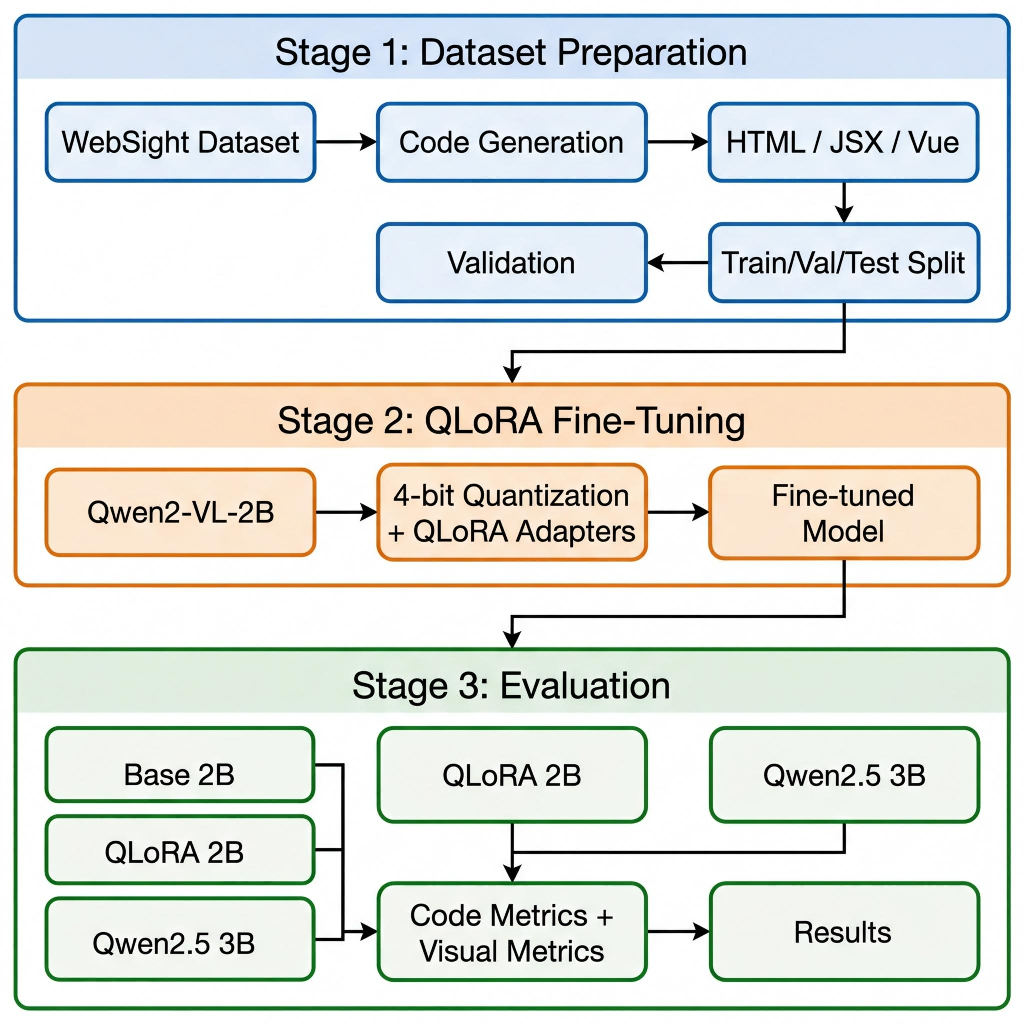
\includegraphics[width=0.88\linewidth]{methodology_diagram_simple.pdf}
    \caption{Pipeline: dataset extension and validation, QLoRA fine-tuning, and evaluation.}
    \label{fig:pipeline}
\end{figure}




\subsection{Model Configuration}

Four models are compared.

\begin{itemize}
    \item \textbf{Qwen2-VL-2B-Instruct (Base):} A 2-billion parameter vision-language model from the Qwen2-VL family, evaluated in zero-shot mode~\cite{qwen2vl}.
    
    \item \textbf{Qwen2-VL-2B-Instruct + QLoRA (Fine-tuned):} The same model, fine-tuned with QLoRA on our extended WebSight dataset (Sec.~\ref{subsec:qlora}).

    \item \textbf{Qwen2.5-VL-3B-Instruct (Base):} A newer, larger model from the Qwen2.5-VL family, evaluated zero-shot to test whether a newer architecture and greater scale can match the fine-tuned model \cite{qwen25vl}.

    \item \textbf{Qwen2.5-VL-3B-Instruct + QLoRA (Fine-tuned):} The 3B model fine-tuned on the same data with the same adapters, which separates the effect of fine-tuning from that of model size. To fit in 8\,GB, it uses the BF16 instead of the FP16 16-bit floating-point format (FP16 overflowed), paged 8-bit AdamW and 16-bit frozen embeddings, and it was trained for one epoch (3,152 steps, about 34\,h) instead of three.
\end{itemize}

\subsection{QLoRA Fine-Tuning Procedure}
\label{subsec:qlora}

Following the low-rank adaptation of Hu \textit{et al.}~\cite{hu2021lora},
the update to a pretrained weight matrix $W_0 \in \mathbb{R}^{d \times k}$ is
constrained to the low-rank form $\Delta W = \frac{\alpha}{r} B A$,
where $A \in \mathbb{R}^{r \times k}$ and $B \in \mathbb{R}^{d \times r}$ are
the only trainable matrices, $r \ll \min(d,k)$ is the adapter rank, and
$\alpha$ is a scaling factor. In QLoRA~\cite{dettmers2023qlora}, the frozen
weights are stored in 4-bit NormalFloat (NF4) with double quantization and
dequantized on the fly during the forward pass:
\begin{equation}
h \;=\; \mathrm{dequant}\!\left(c^{(1)}, c^{(2)}, W^{\mathrm{NF4}}\right) x
\;+\; \frac{\alpha}{r}\, B A x ,
\label{eq:qlora}
\end{equation}
where $c^{(1)}, c^{(2)}$ are the first- and second-level quantization
constants. Adapters of rank $r{=}64$ with $\alpha{=}128$ and dropout $0.05$
are attached to all attention and feed-forward projections (\texttt{q\_proj},
\texttt{k\_proj}, \texttt{v\_proj}, \texttt{o\_proj}, \texttt{gate\_proj},
\texttt{up\_proj}, \texttt{down\_proj}); the adapters are trained in FP16 while
the backbone is kept frozen in NF4.

Training minimizes the causal language-modeling loss
$\mathcal{L}(\theta) = -\sum_{t \in \mathcal{T}_{\mathrm{code}}} \log p_\theta(y_t \mid y_{<t}, I, p)$
for image $I$, prompt $p$ and reference code $y$, where
$\mathcal{T}_{\mathrm{code}}$ indexes only the assistant's code tokens; image
and prompt positions are excluded by label masking, and the vision encoder
receives no adapters.
Optimization uses AdamW with a learning rate of $1{\times}10^{-4}$, 100 warmup
steps, weight decay 0.01, batch size 1 with gradient accumulation 8 (effective
batch 8), and 3 epochs over the 25,215 multi-task training examples, with a
validation pass over the 2,964 validation examples after the final step.
Training sequences (image, prompt and code) are limited to 2,048 tokens, and
gradient checkpointing and FP16 mixed precision keep peak training memory low.
All training and inference ran on one NVIDIA GeForce RTX 3070 Ti (8\,GB).

\subsection{Evaluation Framework}
\label{subsec:eval}

All four models are evaluated on the 1,488 held-out test conversations with
greedy decoding and at most 1,536 new tokens, a limit that covers 99.93\% of
the test references. Metrics are computed
per task (HTML, JSX, Vue) and then averaged, so that no task dominates the
aggregate. Uncertainty is estimated with a paired bootstrap over the 496 test
images (1,000 resamples; 500 for CodeBLEU) that resamples the three tasks of an
image together; $p$-values are two-sided. Three complementary dimensions are measured.

\subsubsection{Code-Level Metrics}
Parse Success Rate (PSR) measures executable syntactic validity as the
fraction of generated outputs accepted by a production-grade parser
(\texttt{@babel/parser} for JSX, \texttt{@vue/compiler-sfc} for Vue).
Similarity to the reference code is measured by BLEU-4 \cite{papineni2002bleu} and its code-aware
extension CodeBLEU \cite{ren2020codebleu} (which adds AST-match and data-flow components and is
computed with a fixed Python hash seed, on which its data-flow match depends); ROUGE-L,
ChrF and METEOR rank the four models as BLEU-4 does and are omitted for
space. Character-level closeness is captured by edit
similarity based on the Levenshtein distance $\mathrm{Lev}(\cdot,\cdot)$:
\begin{equation}
\mathrm{EditSim}(\hat{y}, y) \;=\;
1 - \frac{\mathrm{Lev}(\hat{y}, y)}{\max\!\left(|\hat{y}|, |y|\right)} .
\label{eq:editsim}
\end{equation}
Structure is assessed by tag accuracy (the fraction of reference HTML/JSX tags
recovered in the prediction) and tree edit similarity, computed as in
\eqref{eq:editsim} on the sequences of markup tags rather than characters.

\subsubsection{Visual-Fidelity Metrics}
Each generated component is rendered in a headless Chromium browser
(Playwright) at a 1280$\times$960 viewport: raw HTML is wrapped in a full page
with Tailwind, JSX is mounted as a React component, and the Vue template is
extracted and rendered. Import statements are removed before mounting, so a
component that depends on a third-party UI library fails to render; Section~V
also reports a lenient variant that replaces such library components with plain
\texttt{<div>} stubs. The screenshot of the render is compared against the
original WebSight screenshot. SSIM is computed following
Wang \textit{et al.}~\cite{wang2004ssim}, peak signal-to-noise ratio (PSNR) as
$10\log_{10}(\mathrm{MAX}^2/\mathrm{MSE})$ in dB, with MSE the mean squared error, and
learned perceptual image patch similarity (LPIPS) \cite{zhang2018lpips} from deep AlexNet features (lower is better). Samples whose
code fails to render are not excluded; they receive the worst value of each
metric (zero for SSIM and PSNR, one for LPIPS), so visual scores jointly
reflect renderability and appearance. Because the JSX and Vue references were
produced by Qwen2.5-Coder-7B, code-similarity metrics partly measure agreement
with the teacher's coding style; we therefore treat the visual metrics, which
compare renders with the original screenshot, as the primary measure of output
quality. As an upper bound, the reference code itself reaches SSIM 0.722, PSNR
12.41\,dB and LPIPS 0.492 under the same procedure.

\subsubsection{Real-World Pages}
To test whether the models transfer to real pages, we use Design2Code
\cite{si2025design2code}, 484 real web pages with their HTML. Because the
models were trained on single-screen pages, the input and the comparison target
are the first screen of each page, a 16:9 crop of the top of its screenshot,
downscaled to 640$\times$360 for the model as in WebSight. We evaluate a random
100 pages with the same prompts, decoding and rendering. No JSX or Vue
references exist for these pages, so only visual metrics are reported, and the
real HTML rendered by the same harness gives the upper bound. Because of the crop
and the metrics, the scores are not comparable with those of Si \textit{et al.},
who score full pages by matched blocks, text, position, color and CLIP similarity.



\section{Experimental Results}
\label{sec:results}

Table~\ref{tab:results} reports the results of the four models averaged over the three tasks (HTML, JSX, Vue). The fine-tuned 2B model obtains the best or joint-best value on every metric; on SSIM, it is statistically tied with both 3B models (Section~\ref{subsec:comparison}).

\begin{table}[htbp]
\centering
\caption{Overall performance across all tasks (averaged). Base and Qwen2.5 are zero-shot; QLoRA (3B) is Qwen2.5-VL-3B fine-tuned for one epoch. Best values in bold.}
\label{tab:results}
\footnotesize
\setlength{\tabcolsep}{3pt}
\renewcommand{\arraystretch}{1.1}
\begin{tabular}{lcccc}
\hline
\textbf{Metric} & \textbf{Base} & \textbf{Qwen2.5} & \textbf{QLoRA} & \textbf{QLoRA} \\
 & \textbf{(2B)} & \textbf{(3B)} & \textbf{(2B)} & \textbf{(3B)} \\
\hline
SSIM & 0.509 & 0.711 & \textbf{0.716} & \textbf{0.716} \\
PSNR (dB) & 8.43 & 11.56 & \textbf{12.09} & 11.94 \\
LPIPS $\downarrow$ & 0.681 & 0.563 & \textbf{0.515} & 0.524 \\
\hline
PSR (\%) & 96.24 & 99.46 & \textbf{99.93} & \textbf{99.93} \\
BLEU-4 & 52.24 & 54.31 & \textbf{80.73} & 78.41 \\
CodeBLEU & 0.520 & 0.575 & \textbf{0.735} & 0.713 \\
Edit Sim. & 0.498 & 0.537 & \textbf{0.774} & 0.752 \\
Tag Accuracy & 0.564 & 0.641 & \textbf{0.874} & 0.850 \\
Tree Edit Sim. & 0.507 & 0.532 & \textbf{0.807} & 0.785 \\
\hline
\end{tabular}
\end{table}

\textbf{Efficiency:} A batch finishes only when its longest output does, so we timed every model on the same 24 test samples with batch size 8; outputs averaged 347 to 433 tokens, and none reached the limit. Per sample, QLoRA (2B) needs 11.2\,s and 2.18\,GiB of peak GPU memory, the base model 6.4\,s and 4.59\,GiB, QLoRA (3B) 12.9\,s and 3.30\,GiB, and the zero-shot 3B model 22.9\,s and 6.47\,GiB. QLoRA thus halves the memory of its base model and is twice as fast as the zero-shot 3B model, but it is 1.75$\times$ slower than the 16-bit base model. This agrees with the dequantization overhead reported for QLoRA models \cite{huang2024llama3quant}; the separately applied adapter probably adds to it.






  
\begin{table}[t]
\centering
\caption{Per-task performance for selected metrics.}
\label{tab:per_task}
\footnotesize
% \usepackage{} 


\resizebox{\columnwidth}{!}{
\begin{tabular}{llcccc}
\toprule
\textbf{Task} & \textbf{Metric} & \textbf{Base (2B)} & \textbf{Qwen2.5 (3B)} & \textbf{QLoRA (2B)} & \textbf{QLoRA (3B)} \\
\midrule
HTML & PSR (\%) & 100.0 & 100.0 & 100.0 & 100.0 \\
 & BLEU-4 & 64.69 & 59.16 & 83.23 & 81.01 \\
 & CodeBLEU & 0.639 & 0.607 & 0.773 & 0.750 \\
 & SSIM & 0.724 & 0.717 & 0.752 & 0.748 \\
 & Rendered (\%) & 96.4 & 97.8 & 100.0 & 100.0 \\
\midrule
JSX & PSR (\%) & 94.76 & 98.79 & 100.0 & 99.80 \\
 & BLEU-4 & 38.86 & 50.46 & 81.32 & 78.52 \\
 & CodeBLEU & 0.462 & 0.527 & 0.703 & 0.680 \\
 & SSIM & 0.099 & 0.697 & 0.690 & 0.690 \\
 & Rendered (\%) & 12.1 & 95.2 & 100.0 & 99.8 \\
\midrule
Vue & PSR (\%) & 93.95 & 99.60 & 99.80 & 100.0 \\
 & BLEU-4 & 53.16 & 53.31 & 77.64 & 75.70 \\
 & CodeBLEU & 0.460 & 0.590 & 0.728 & 0.709 \\
 & SSIM & 0.703 & 0.720 & 0.706 & 0.710 \\
 & Rendered (\%) & 98.0 & 99.4 & 100.0 & 100.0 \\
\bottomrule
\end{tabular}
}
\end{table}
Table~\ref{tab:per_task} gives the per-task breakdown. \textbf{HTML} is the easiest task, with 100\% PSR for all models. \textbf{JSX} shows the largest gap: QLoRA's BLEU-4 is 109\% higher than the base model's (81.32 vs.\ 38.86), and the difference is largest in renderability: all 496 QLoRA outputs render in a browser, against 95.2\% for the zero-shot 3B model and only 12.1\% for the base model. The base model's failures come almost entirely from library imports: 437 of its 496 JSX outputs import a UI library such as react-bootstrap despite the Tailwind-only instruction, against 19 for the zero-shot 3B model and none for QLoRA. With these imports replaced by stubs, 87.7\% of the base model's JSX outputs render (SSIM 0.638, LPIPS 0.624), so the strict renderability gap mostly reflects instruction following rather than broken layouts. \textbf{Vue} follows a similar pattern: QLoRA improves BLEU-4 by 46\% and reduces parse failures from about 6\% to 0.20\%.



\subsection{Model Comparison}
\label{subsec:comparison}

\textbf{QLoRA vs. base model:} Fine-tuning the 2B model raises BLEU-4 from 52.24 to 80.73 (+54.5\%) and CodeBLEU from 0.520 to 0.735 (+41.3\%), and all three visual metrics improve significantly under the strict harness (paired bootstrap, $p<0.01$), with SSIM rising from 0.509 to 0.716. With the base model's library imports stubbed, the gap narrows to 0.027 SSIM and 0.064 LPIPS, so much of the strict visual gain comes from renderability.

\textbf{QLoRA vs. Qwen2.5-VL-3B:} With fewer parameters, the fine-tuned 2B model exceeds the zero-shot 3B model on code similarity (CodeBLEU +0.160, 95\% confidence interval (CI) [0.151, 0.169]; BLEU-4 +26.4) and on perceptual similarity (LPIPS $-0.048$ [$-0.057$, $-0.040$]; PSNR +0.53\,dB [0.29, 0.77]). The SSIM difference (+0.005 [$-0.004$, 0.014], $p=0.33$) is not significant, and on Vue the zero-shot 3B model has a significantly higher SSIM (0.720 vs.\ 0.706); for models that render reliably, SSIM is close to its 0.722 ceiling, which limits its ability to separate them.

\textbf{QLoRA (2B) vs. QLoRA (3B):} Fine-tuning closes most of the 3B model's gap to the fine-tuned 2B model, raising its BLEU-4 from 54.31 to 78.41 and lowering its LPIPS from 0.563 to 0.524, but it does not overtake it. The two are tied on SSIM ($-0.0004$ [$-0.005$, 0.004], $p=0.87$), and the 2B model is slightly better on LPIPS ($-0.009$ [$-0.015$, $-0.003$]), PSNR (+0.15\,dB [0.01, 0.30]), BLEU-4 (+2.3 [1.6, 3.0]) and CodeBLEU (+0.022 [0.015, 0.028]). QLoRA (3B) was trained for one epoch instead of three and in BF16 instead of FP16; at this budget, the larger model brings no gain while needing 51\% more GPU memory and 15\% more time per sample.

\textbf{Summary:} QLoRA fine-tuning of the 2B model gives the highest code validity (PSR 99.93\%, equal to QLoRA (3B)), is the only configuration whose outputs all render on every task, and has the best LPIPS and PSNR, with SSIM tied with both 3B models. Because the baselines are zero-shot or fine-tuned with the same method, these results show the benefit of in-domain fine-tuning, which QLoRA makes affordable on an 8\,GB GPU; they do not show that QLoRA is better than other ways of adapting a model.

\subsection{Real-World Pages}
\label{subsec:d2c}

\begin{table}[t]
\centering
\caption{Visual fidelity on 100 random Design2Code pages (first screen), averaged over HTML, JSX and Vue. Rendered: outputs that render, per task. $^*$First 25 pages only.}
\label{tab:d2c}
\footnotesize
\setlength{\tabcolsep}{3.5pt}
\renewcommand{\arraystretch}{1.1}
\begin{tabular}{lcccc}
\hline
\textbf{Model} & \textbf{SSIM} & \textbf{PSNR} & \textbf{LPIPS}$\downarrow$ & \textbf{Rendered (\%)} \\
 & & \textbf{(dB)} & & \textbf{H / J / V} \\
\hline
Real HTML (bound) & 0.686 & 11.02 & 0.507 & 94 / -- / -- \\
Base (2B) & 0.458 & 6.78 & 0.753 & 96 / 13 / 90 \\
QLoRA (2B) & 0.668 & 9.99 & 0.631 & 100 / 93 / 99 \\
QLoRA (3B) & 0.667 & 9.99 & 0.617 & 100 / 98 / 99 \\
\hline
Qwen2.5 (3B)$^*$ & 0.627 & 9.16 & 0.650 & 100 / 88 / 100 \\
QLoRA (2B)$^*$ & 0.607 & 9.25 & 0.639 & 100 / 88 / 96 \\
\hline
\end{tabular}
\end{table}

All scores drop on real pages (Table~\ref{tab:d2c}), but fine-tuning still helps. QLoRA (2B) improves on its base model by 0.210 SSIM [0.183, 0.239], 3.2\,dB PSNR and 0.122 LPIPS (paired bootstrap over pages, all $p<0.001$); the gain is largest for JSX (SSIM 0.623 vs.\ 0.094; all 87 failed base renders import a UI library) but also holds for HTML (0.714 vs.\ 0.668) and Vue (0.669 vs.\ 0.613). QLoRA (2B) is tied with QLoRA (3B) on all three metrics ($p \ge 0.08$). Six real pages fail to render even from their own HTML; on the other 94, the real HTML reaches SSIM 0.730 and QLoRA's HTML 0.716. On the 25 pages also given to the zero-shot 3B model, QLoRA (2B) is statistically tied with it (SSIM $-0.021$ [$-0.071$, 0.032], LPIPS $-0.012$ [$-0.052$, 0.027]), so its LPIPS advantage on WebSight is not confirmed on real pages, although 25 pages give little statistical power. The main weakness is output length: the fine-tuned model writes about 600 tokens per page, the scale of its WebSight training targets (459 on average), whereas the real HTML has a median of 14,805 tokens, much of it scripts, metadata and styles that are not visible; output length is unrelated to page length ($r=0.05$). The base model reaches the 1,536-token limit in 41 of its 300 outputs, 29 of them repetition loops, against 4 for QLoRA (2B).

% % \begin{figure*}[t]
% % \centering
% % \includegraphics[width=\textwidth]{}
% % \caption{Proposed Pipeline}
% % \end{figure*}
% \begin{figure}[h]
% \centering
% \includegraphics[width=0.95\linewidth]{radar_comparison.pdf}
% \caption{ Radar chart showing normalized performance comparison across key metrics}
% \end{figure}

\section{Error Analysis and Discussion}

\textbf{Syntax and structure:} QLoRA almost eliminates syntax errors (0\% for JSX, 0.2\% for Vue), and only 3.2\% of its outputs are far from the reference structure (edit similarity $<0.3$), compared with 18.7\% for the base model.

\textbf{Failure modes:} The two zero-shot models often produce a different element structure for the same layout (tree edit similarity 0.507 and 0.532, against 0.807 for QLoRA), and the zero-shot 3B model adds a style block or inline styles to 280 of its 496 HTML pages, against 109 of the reference pages. QLoRA, in contrast, follows the syntax of the reference code closely, and none of its WebSight outputs reaches the 1,536-token limit.

\textbf{Teacher circularity:} BLEU-4 and CodeBLEU partly reward the coding style of Qwen2.5-Coder-7B, which the fine-tuned model also learns (Section~\ref{subsec:eval}); four results limit this concern. First, the HTML references are the original WebSight code, which our teacher did not produce, and QLoRA still raises HTML BLEU-4 from 64.69 to 83.23. Second, the visual metrics compare renders with the original screenshot rather than with the teacher's code; on them, QLoRA reaches 99\% of the reference code's SSIM and covers two-thirds of the LPIPS distance between the zero-shot 3B model and the reference code. Third, the render-based check in Section~\ref{subsec:data-quality-validation} shows that the teacher's targets reproduce their source pages. Fourth, on Design2Code, for which no teacher code exists, fine-tuning still improves every visual metric (Section~\ref{subsec:d2c}).

\textbf{Model size:} QLoRA (3B) had a lower training loss than QLoRA (2B) at the same steps of the first epoch (0.053 vs.\ 0.061 over its last 100 steps), yet it scored lower on the test set. Because the 2B model was trained for two further epochs, the larger model may be under-trained rather than less suited to the task; we did not test this.




\section{Conclusion and Limitations}

This paper presented a pipeline for generating framework-native code from UI
screenshots. We extended the WebSight dataset with more than 15,000
parser-validated React JSX and Vue 3 SFC equivalents of synthetic HTML pages, and
used it to fine-tune a 2B-parameter vision-language model with QLoRA. On the
WebSight test set, the fine-tuned model reaches a PSR of 99.93\%, renders on
every task, and exceeds the zero-shot 3B model on code similarity, LPIPS and
PSNR while using a third of its GPU memory; on SSIM the two are statistically tied. The 3B model fine-tuned with the
same recipe did not surpass it, and on 100 real Design2Code pages fine-tuning
kept a large advantage over the base model. These results indicate that, for
this task, in-domain fine-tuning of a small model can match a larger fine-tuned
model and, on WebSight-style pages, outperform a larger model used zero-shot.
Running on a consumer GPU, the model avoids per-token API cost, keeps unreleased
designs on-premises and serves HTML, React and Vue from one deployment; its
output should still be reviewed before it is merged.

The study has several limitations. First, the training data are synthetic
WebSight pages, which lack the dynamic states, state management, accessibility
requirements and structural complexity of production interfaces; on real pages,
the fine-tuned model writes far shorter code than the originals, its SSIM
falls from 0.716 to 0.668, and on 25 pages it is statistically tied with the
zero-shot 3B model. Second, the JSX and Vue references come from a
single teacher model, so code-similarity metrics partly reward its style. Third,
the visual metrics use static screenshots and do not measure interaction or
responsiveness. Fourth, each configuration was trained once, and QLoRA (3B)
for one epoch and in BF16, so neither run-to-run variance nor the effect of
these differences is measured. Fifth, the
1,536-token limit truncated 3.7\% of the base model's and 1.1\% of the zero-shot
3B model's WebSight outputs, though none of QLoRA's. Finally, GPU memory limited
the comparison with other adaptation techniques and the length of the training
sequences.

In future work, we will compare QLoRA with LoRA and DoRA \cite{liu2024dora} on
the same hardware, train on longer real-world pages such as those of WebCode2M
\cite{gui2025webcode2m}, add interaction-aware metrics, and add an
inference-time self-repair loop driven by validation errors.


% \section*{Limitations} This section projects different shortcomings that caused obstructions during the investigation of different ML, DL, and Transformer-based models for Subtask 1 and Subtask 2. 
% \begin{itemize}
% \item One of the limitations of this system is that it applies to only the Malayalam language. For other languages, a different system with different preprocessing has to be used. 
% \item Another limitation is the number of classes dataset of subtask-2, for fine grained classification number of classes increased. Because of the increased classes result dropped a bit.
% \item Texts with portions written in different languages are another limitation. Because it can not be trained properly as our system works only for the Malayalam language.
% \end{itemize}

%% The ACL source had BOTH a manual thebibliography (b1-b6, never cited by
%% any \cite{}) AND \bibliography{custom}, which produced two References
%% sections. The phantom list is dropped; all 36 citations resolve via custom.bib.
\bibliographystyle{IEEEtran}
\bibliography{custom}

\end{document}
